\section{Parallelism and Concurrency Basics}

\begin{definition}{Important Definitions}
    \begin{itemize}
        \item \textbf{Parallelism:} Multiple processes or threads executing simultaneously
        \item \textbf{Concurrency:} Multiple processes or threads making progress independently
        \item \textbf{Mutual Exclusion:} Ensures that only one thread accesses a resource at a time
        \item \textbf{Synchronization:} Mechanisms to control the order of execution of threads
        \item \textbf{Critical Section:} A part of code that accesses shared resources and must not be executed by more than one thread at a time
        \item \textbf{Deadlock:} A situation where two or more threads are blocked forever, waiting for each other
        \item \textbf{Livelock:} A situation where threads are continuously changing states without making progress
        \item \textbf{Starvation:} A thread is perpetually denied access to a resource it needs for execution
        \item \textbf{Locks and Semaphores:} Tools to manage access to shared resources
        \item \textbf{Condition Variables:} Used for signaling between threads
    \end{itemize}
\end{definition}

\begin{concept}{Famous Problems}
    \begin{itemize}
        \item \textbf{Producer-Consumer Problem:} Managing a shared buffer between producer and consumer threads
        \item \textbf{Reader-Writer Problem:} Allowing multiple readers or one writer to access a shared resource
        \item \textbf{Dining Philosophers Problem:} Managing resource sharing among multiple threads with potential deadlock
        \item \textbf{Sleeping Barber Problem:} Synchronizing access to a barber shop with limited resources
    \end{itemize}
\end{concept}

\subsection{Process States}

\begin{concept}{Process States} (for details see a few pages ago)
    \begin{itemize}
        \item New: Process is being created
        \item Ready: Process is waiting to be assigned to a processor
        \item Running: Instructions are being executed
        \item Waiting: Process is waiting for some event to occur (e.g., I/O completion)
        \item Terminated: Process has finished execution
    \end{itemize}
\end{concept}

\begin{KR}{Process State Analysis}
    \paragraph{State identification}
    \begin{itemize}
        \item Running: Has CPU, actively executing
        \item Ready: Waiting for CPU only
        \item Blocked: Waiting for external event/resource
        \item Additional states: Swapped, Zombie, Created
    \end{itemize}
    
    \paragraph{Transition triggers}
    \begin{itemize}
        \item Timer interrupts (quantum expiration)
        \item I/O operations (blocking)
        \item System calls
        \item Resource availability
        \item Scheduler decisions
    \end{itemize}
\end{KR}

\begin{example2}{Process State Transitions}
    Name and explain the three main states processes can transition between:
    \vspace{1mm}\\
    \textbf{The three fundamental process states:}
    \begin{itemize}
        \item \textbf{Running}: Process is currently executing on CPU
        \item \textbf{Ready}: Process is ready to execute, waiting for CPU assignment
        \item \textbf{Blocked/Sleeping}: Process cannot execute, waiting for an event (e.g., I/O completion)
    \end{itemize}
    
    \textbf{State transitions:}
    \begin{itemize}
        \item Ready $\rightarrow$ Running: Scheduler assigns CPU
        \item Running $\rightarrow$ Ready: Time quantum expires or preemption
        \item Running $\rightarrow$ Blocked: Process waits for I/O or resource
        \item Blocked $\rightarrow$ Ready: Awaited event occurs
    \end{itemize}
\end{example2}

\subsection{Resource Graphs}

\begin{example2}{Resource Graph Analysis}\\
    Ein Rechnersystem besitzt zwei Tapestationen (T1, T2) und zwei Disks (D1, D2). Zur Zeit laufen drei Prozesse (P1, P2, P3), wobei folgendes gilt:
    \begin{itemize}
        \item Prozess P1 kopiert Daten von Disk D1 auf die Tapestation T2 und möchte Daten auf den Disk D2 schreiben
        \item Prozess P2 hat Tapestation T1 alloziert und möchte Daten auf Disk D2 schreiben
        \item Prozess P3 hat Disk D2 alloziert und möchte Daten nach Tapestation T2 kopieren
    \end{itemize}
    
    Ist das eine Deadlocksituation, wenn die Ressourcen exklusiv alloziert werden und wenn möchte schreiben das Gleiche wie anfordern bedeutet? Begründen Sie Ihre Antwort (Ressourcengraphen zeichnen und analysieren).
    
    \tcblower

    \begin{minipage}{0.4\linewidth}
        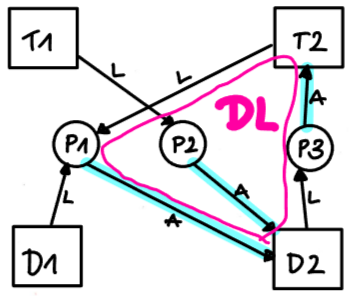
\includegraphics[width=\linewidth]{deadlock_resource_graph.png}
    \end{minipage}
    \begin{minipage}{0.58\linewidth}    
    \textbf{Analyse:}
    \begin{itemize}
        \item P1 hält D1, möchte T2 und D2
        \item P2 hält T1, möchte D2  
        \item P3 hält D2, möchte T2
    \end{itemize}
    
    Es entsteht ein Zyklus: P1 $\rightarrow$ D2 $\rightarrow$ P3 $\rightarrow$ T2 $\rightarrow$ P1\\
    
    \textbf{Bedingungen für Deadlock:}
    \begin{itemize}
        \item Mutual Exclusion: Ressourcen werden exklusiv alloziert
        \item No Preemption: Ressourcen können nicht weggenommen werden
        \item Hold \& Wait: Prozesse halten Ressourcen und warten auf weitere
        \item Circular Wait: Es gibt einen Zyklus im Ressourcengraph
    \end{itemize}
    
    Alle vier Bedingungen sind erfüllt $\rightarrow$ Deadlock!
    \end{minipage}
\end{example2}

\raggedcolumns

\begin{KR}{Deadlock Detection in Resource Allocation Graphs}
    \paragraph{Resource Graph erstellen}
    \begin{itemize}
        \item Kreise: Prozesse (P1, P2, P3, ...)
        \item Rechtecke: Ressourcen (R1, R2, R3, ...)
        \item Pfeile von Prozess zu Ressource: Reqüst (Anforderung)
        \item Pfeile von Ressource zu Prozess: Allocation (Zuteilung)
    \end{itemize}
    
    \paragraph{Deadlock-Analyse}
    \begin{itemize}
        \item Suche nach Zyklen im Graph
        \item Ein Zyklus bedeutet Deadlock bei Single-Instance Ressourcen
        \item Bei Multi-Instance Ressourcen: Prüfe ob alle Instanzen blockiert
    \end{itemize}
    
    \paragraph{Deadlock-Bedingungen prüfen}
    \begin{itemize}
        \item Mutual Exclusion: Exklusive Ressourcennutzung
        \item Hold \& Wait: Halten und gleichzeitig warten
        \item No Preemption: Keine Unterbrechung möglich
        \item Circular Wait: Zyklische Warteabhängigkeiten
    \end{itemize}
    
    \paragraph{Lösungsansätze}
    \begin{itemize}
        \item Prevention: Eine der vier Bedingungen verhindern
        \item Avoidance: Banker's Algorithm
        \item Detection \& Recovery: Deadlock erkennen und auflösen
    \end{itemize}
\end{KR}

\raggedcolumns
\columnbreak

\subsection{Synchronization with Semaphores}

\begin{KR}{Synchronization Problem Solving}
    \begin{itemize}
        \item Identify critical sections
        \item Determine synchronization requirements
        \item Choose appropriate mechanism (mutex, semaphore, monitor)
        \item Ensure deadlock avoidance
        \item Test for race conditions
    \end{itemize}
\end{KR}


\begin{concept}{Semaphores}
    \begin{itemize}
        \item Semaphores are synchronization primitives used to control access to shared resources.
        \item They can be binary (0 or 1) or counting (any non-negative integer).
        \item Operations: 
            \begin{itemize}
                \item \texttt{wait(S)}: Decrement the semaphore S. If S is less than 0, block the process.
                \item \texttt{signal(S)}: Increment the semaphore S. If S was negative, wake up a blocked process.
            \end{itemize}
    \end{itemize}
\end{concept}

\begin{KR}{Semaphore-basierte Synchronisation}
    \paragraph{Semaphore verstehen}
    \begin{itemize}
        \item Semaphore S ist ein Zähler mit atomaren Operationen
        \item down(S) oder P(S): Dekrementiert S, blockiert bei S $\leq$  0
        \item up(S) oder V(S): Inkrementiert S, weckt wartende Prozesse
        \item Initialisierung bestimmt verfügbare Ressourcen
    \end{itemize}
    
    \paragraph{Synchronisationsmuster}
    \begin{itemize}
        \item Mutual Exclusion: Binary Semaphore (0/1) um kritische Bereiche
        \item Signaling: Ein Prozess signalisiert einem anderen (Producer-Consumer)
        \item Rendezvous: Zwei Prozesse warten aufeinander
        \item Barrier: Mehrere Prozesse warten aufeinander
    \end{itemize}
    
    \paragraph{Typische Synchronisationsprobleme}
    \begin{itemize}
        \item Producer-Consumer: Buffer-Management mit vollen/leeren Plätzen
        \item Reader-Writer: Mehrere Leser oder ein Schreiber
        \item Dining Philosophers: Deadlock-Vermeidung bei zyklischen Abhängigkeiten
        \item Barrier Synchronization: Alle warten aufeinander
    \end{itemize}
    
    \paragraph{Implementierungsschritte}
    \begin{itemize}
        \item Identifiziere Synchronisationspunkte
        \item Bestimme benötigte Semaphore und deren Initialisierung
        \item Verwende down() vor kritischen Bereichen/Warten
        \item Verwende up() nach kritischen Bereichen/Signaling
        \item Teste auf Deadlock-Freiheit und korrekte Reihenfolge
    \end{itemize}
\end{KR}

\begin{example2}{Semaphore Implementation}\\
    Gegeben sind drei Prozess P0, P1, und P2 die nach folgendem Schema abgearbeitet werden soll:\\
    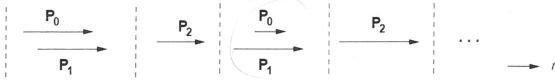
\includegraphics[width=0.8\linewidth]{semaphore_mt12.png}
    
    Die Verarbeitung startet mit den beiden Prozessen P0 und P1, die parallel verarbeitet werden sollen (es spielt kein Rolle, welcher der beiden Prozesse zürst mit seiner Verarbeitung beginnt oder aufhört). Wenn beide Prozesse eine Iteration ihrer Funktion working(x) beendet haben, folgt Prozess P2, etc.
    
    Schreiben Sie Pseudocode mit maximal 3 Semaphoren S0, S1 und S2, der garantiert, dass die oben skizzierte Reihenfolge eingehalten wird. Verwenden Sie dazu ausschliesslich Befehle der Form up(S0) und down(S0), etc. Geben Sie an, wie die Semaphore initialisiert werden müssen.
    
    \tcblower

    \begin{minipage}{0.56\linewidth}
    
    \begin{center}
    \begin{tabular}{|l|l|l|}
    \hline
    \textbf{P0} & \textbf{P1} & \textbf{P2} \\
    \hline
    Sem S0: 1 &  & \\
    Sem S1: 1 &  & \\
    Sem S2: 0 &  & \\
    \hline
    while(1) \{ & while(1) \{ & while(1) \{ \\
    \quad \quad down(S0); & \quad \quad down(S1); & \quad \quad down(S2); \\
    \quad \quad working(0); & \quad \quad working(1); & \quad \quad working(2); \\
    \quad \quad up(S2); & \quad \quad up(S2); & \quad \quad up(S0); \\
    \} & \} & \quad \quad up(S1); \\
     &  & \} \\
    \hline
    \end{tabular}
    \end{center}
    \end{minipage}
    \begin{minipage}{0.42\linewidth}
    
    \textbf{Initialisierung:}
    \begin{itemize}
        \item S0 = 1 (P0 kann starten)
        \item S1 = 1 (P1 kann starten) 
        \item S2 = 0 (P2 muss warten - Synchronisation zwischen P0/P1 und P2)
    \end{itemize}
    
    \textbf{Ablauf:}
    \begin{itemize}
        \item P0 und P1 starten parallel
        \item Beide signalisieren mit up(S2) wenn fertig
        \item P2 wartet mit down(S2) bis beide P0 und P1 fertig sind
        \item P2 gibt mit up(S0) und up(S1) die nächste Runde frei
    \end{itemize}
    \end{minipage}
\end{example2}

\subsubsection{Producer-Consumer Problem}

\begin{KR}{Producer-Consumer pattern}
    \begin{itemize}
        \item Identify shared resource (buffer)
        \item Determine capacity constraints
        \item Create semaphores for available/used slots
        \item Producer: wait(empty), produce, signal(full)
        \item Consumer: wait(full), consume, signal(empty)
    \end{itemize}
\end{KR}


\begin{example2}{Producer-Consumer Problem}
    Implement a semaphore-based solution for the producer-consumer problem:

    \begin{minipage}{0.56\linewidth}

\begin{lstlisting}[language=C, style=basesmol]
const int N = 4;      // Maximum buffer size
int sem_write = N;    // Semaphore for write slots
int sem_read = 0;     // Semaphore for read slots

// Producer process
while(1) {
    wait(sem_write);  // Wait for empty slot
    write(value);     // Write to buffer
    signal(sem_read); // Signal data available
}

// Consumer process  
while(1) {
    wait(sem_read);   // Wait for data
    read(value);      // Read from buffer
    signal(sem_write);// Signal slot available
}
\end{lstlisting}
    \end{minipage}
    \hspace{2mm}
    \begin{minipage}{0.4\linewidth}
    \textbf{Key points:}
    \begin{itemize}
        \item sem\_write tracks empty buffer slots
        \item sem\_read tracks filled buffer slots
        \item Producer waits for empty slots, signals filled slots
        \item Consumer waits for filled slots, signals empty slots
    \end{itemize}
    \end{minipage}
\end{example2}


